% #############################################################################
% This is Chapter 4
% !TEX root = ../main.tex
% #############################################################################
% Change the Name of the Chapter i the following line
\fancychapter{Algorithmic Optimization}
\cleardoublepage
% The following line allows to ref this chapter
\label{chap:implement}

In the last chapter, we discussed the architecture of the proposed solution, a general purpose optimization framework that is applicable to solve any optimization problem. 

From the beginning, we set out to address optimization problems involving costly functions. Therefore, during the development of the prototype of the proposed framework we focused on problems that exhibited these properties. Nevertheless, that the prototype can be easily extended to include other algorithms (e.g., derivative-based), as it has been previously discussed in ~\Cref{sec:optalgos}. 

Motivated by the large impact of the building sector in the world's sustainability and economy, this dissertation aims at applying the proposed framework to address building design optimization, thus attempting to reduce the costs and ecological footprint of buildings. Despite the existence of of multiple optimization tools in architecture (see~\Cref{sec:plugins}), these are often limited and do not provide adequate algorithms, nor mechanisms to enable the efficient optimization of problems with time-consuming evaluations (see~\Cref{sec:problemsaddress}).

In this chapter, we describe how the general-purpose framework proposed in this dissertation can be applied to address architectural design optimization. 

\section{Algorithmic Optimization}

In \Cref{ssec:ad,ssec:aa}, we have discussed how architectural paradigms have incrementally grown to develop the mechanisms to quickly (1) update a design, (2) generate the corresponding analytical model, and (3) automatically evaluate the design in an analytical tool and collect its results. 

These mechanisms laid down the foundations for automated optimization processes. By extending the Algorithmic Design (AD) and Algorithmic Analysis (AA) approaches to include optimization mechanisms, we are able to automatically apply optimization processes that aim to improve (or even optimize) a design’s performance. Using this approach, which we name \ac{AO}, architects are able to optimize their designs through (1) the creation of \ac{AD} models reflecting their design's intents, (2) the selection of the performance aspects to optimize and, thus, the analysis tools to be used (e.g., lighting, thermal, structural, costs), and, finally, (3) of the optimization parameters (e.g., algorithm, algorithm's parameters). In the end, architects must specify not only the design parameters that are to be optimized and their acceptable range of values, but also which analysis to consider for optimization\footnote{\ac{AO} will treat the analysis' results for different variations of the design as the functions to optimize.}. 

- Dizer q durante o processo anterior, user não tem q se preocupar com comunicação entre os diferentes módulso
- Q a ideia será integrar a framework proposa no worfklow descrito
- Q essa integração não altera o workflow, apenas adicionando o facto de q o utilizador tem de passar a especificar os parametros da otimização
- Gestao e comunicação entre os diferentes componentes é gerido pela ferramenta de \ac{AD}

- Ligar c/ práticas já existentes q apresentam limitações, mas que a framework poderá ajudar a ultrapassar algumas com as features enunciadas no capitulo anterior : 


% Currently available architectural optimization frameworks present limitations, as discussed in \Cref{sec:problemsaddress}. This dissertation addresses some of the identified gaps, by connecting the the proposed optimization framework to an \ac{AD} tool, and by adopting the \ac{AD} and \ac{AA} approaches, as depicted in \Cref{fig:algorithmicoptimization}. \todo{Que nível de detalhe  é preciso colocar aqi? Copiar o do guilherme é simplesmente foleiro xD}



\begin{figure}[htbp]
	\centering
	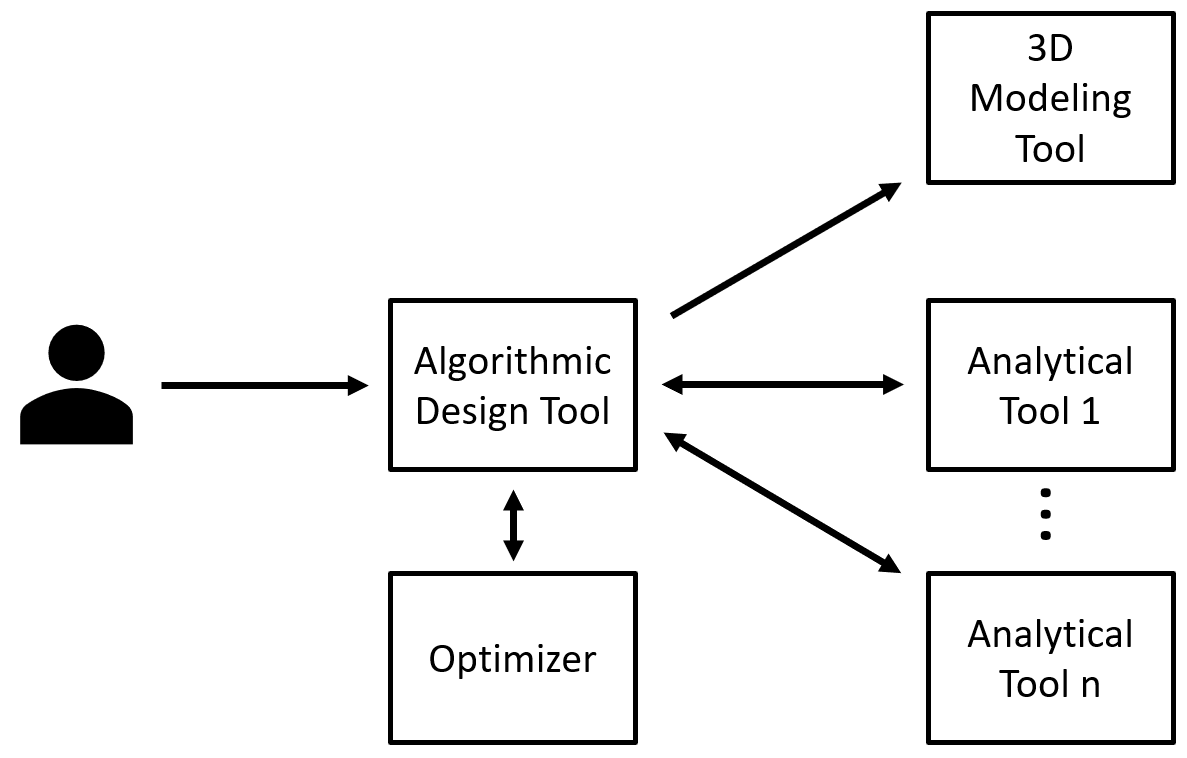
\includegraphics[width=0.6\textwidth]{./Images/Solution/algorithmic_optimization.png}
	\caption{Algorithmic Optimization workflow. In this workflow, the user only interacts with an \ac{AD} tool to create the initial design, to specify the analysis tools, and to specify the optimization parameters.}
	\label{fig:algorithmicoptimization}
\end{figure}

By coupling the framework discussed in \Cref{chap:architecture} with the algorithmic workflow, architects are able to easily apply optimization algorithms to optimize their designs, with the benefit of having algorithms capable of efficiently handling Building Performance Optimization (\ac{BPO}) problems. Besides algorithms, this framework enables them to easily compare different algorithms, providing not only a set of quality indicators for each algorithm, but also a set of different views regarding the distribution and representativeness of the obtained results. As a result, architects can further explore the generated visual representations of the optimization's results and generate the corresponding design variants, using the \ac{AD} tool. 

The visual aspect is important to enhance the comprehension of an optimization run and to the making of more informed decisions. Moreover, using this framework, users are able to visualize close to optimal solutions which may be more suitable to the architects intentions. 


\section{Optimization Benchmarks in Architecture}

\todo{example?}


At the light of the architectural practice, our solution makes use of the textual programming paradigm and, consequently, has a special affinity with textual \ac{AD} tools (e.g., Khepri). As a result, when coupled with these \ac{AD} tools, our solution also benefits from their portability and scalability properties. We aim at reducing the abnormal time-complexity of \ac{BPO} by providing model-based algorithms. 

Finally, we consider the complexity of our solution. Unlike the analyzed tools, our solution does not benefit from the visual paradigm, which means that it should be simple to use and intuitive, even for non-programmers. As a result, we hide the complexity of the integration of optimization libraries under an abstraction layer, providing a clean and succinct set of primitives. These primitives draw inspiration from simple optimization mathematical models and should be rather intuitive and easy to use. 



